\documentclass[12pt,a4paper]{elex2017}
\usepackage[left=2.5cm,right=2.5cm,bottom=2.5cm,top=2.5cm]{geometry}
\usepackage[english]{babel}
\usepackage[T1]{fontenc}
\usepackage[utf8]{inputenc}
\usepackage[unicode=true]{hyperref}
\usepackage{graphicx}
\usepackage[
    style=authoryear,
    natbib=true,
    defernumbers=true
]{biblatex}
\addbibresource{elex-ontolex.bib}

\setcounter{secnumdepth}{3}
\let\subparagraph\paragraph
%\let\subparagraph\relax

% numbering of sections, format of the title
\makeatletter
% we use \prefix@<level> only if it is defined
\renewcommand{\@seccntformat}[1]{%
  \ifcsname prefix@#1\endcsname
    \csname prefix@#1\endcsname
  \else
    \csname the#1\endcsname\quad
  \fi}
\newcommand\prefix@section{\thesection. }
\makeatother

\setlength{\parindent}{0cm}
\setlength{\parskip}{11pt plus 1pt minus 2pt}
\setlength{\bibhang}{1cm}
\setlength{\baselineskip}{16pt}

%\pagestyle{empty}

%%%%%%%%%%%%%%%%%%%%%%%%%%%%%%%%%%%%%%%%%%%%%%%%%%%%%%%%%%%%%%%%%%%%%%%%%%%%%%%%
% DOCUMENT BODY
%%%%%%%%%%%%%%%%%%%%%%%%%%%%%%%%%%%%%%%%%%%%%%%%%%%%%%%%%%%%%%%%%%%%%%%%%%%%%%%%

\begin{document}
\mainmatter
\title{The OntoLex-Lemon Model: development and applications}
\titlerunning{The OntoLex-Lemon Model}
\author{\bf John P. McCrae$^1$, Paul Buitelaar$^1$, Philipp Cimiano$^{2}$}
\institute{$^1$Insight Centre for Data Analytics, National University of Ireland
Galway\\ $^2$ Cognitive Interaction Technology Excellence Cluster, Bielefeld
University\\
E-mail: john@mccr.ae, paul.buitelaar@insight-centre.org,
cimiano@cit-ec.uni-bielefeld.de}
\toctitle{The OntoLex-Lemon Model: development and applications}

\maketitle

\begin{abstract}
Each article must include an abstract of 150 to 200 words in Latin Modern Roman
11 pt with interlinear spacing of 12 pt. The heading Abstract should be
centered, font Times 10 bold. This short abstract will also be used for
printing a Booklet of Abstracts containing the abstracts of all papers
    presented at the Conference.

\keywords{provide 3--5 keywords, separated by semi-colons}
\end{abstract}


% 25,000-50,000 Charcters = 8-15 pages

%The lemon Model, first proposed in~\cite{mccrae2012interchanging}, has become the primary
%model for the representation of lexical data on the Semantic Web and has been
%further developed in the context of the W3C OntoLex Community Group. In this
%paper we will present the development and future outlooks for this model as well
%as briefly detailing some of the current applications of the model. After the
%lemon model was developed in the context of the Monnet project, it was decided
%that the further development of this model should take place within a forum as
%open as possible, which fortunately coincided with the creation of community
%groups for W3C. The community group structure provided mailing lists and wikis
%for discussion of the model and eventually led to the publishing of the model as
%a W3C Report (\cite{cimiano2016lexicon}) and as files in the W3C namespace. The
%discussions within the group covered all aspects of the model, however the issue
%of semantics was of particular interest to the group and led to a major
%innovation in the introduction of a lexical concept, as a distinct element from
%the ontology reference. The formal distinction between these is that an ontology
%reference is an entity in an ontology, which the word denotes.  As such, the
%(ontological) meaning of  the question “When did Prince die?” could be
%understood with the ontology predicate deathDate as a reference, but the general
%concept of dying refers to an event rather than to a date. This also further
%extends the application domain of OntoLex-Lemon, from formal applications such
%as question answering and semantic parsing to the representation of general
%machine-readable dictionaries, including WordNet and digitized versions of
%existing dictionaries.
%Thus, the OntoLex-Lemon model has continued to expand in its use cases and we
%consider two particular cases here. Firstly, the OntoLex-Lemon model has been
%adopted in a variety of online dictionaries and this has provided a common
%interface to these dictionaries. This can be exploited to provide a single
%access point across multiple dictionaries that is implemented in the back-end by
%means of generic SPARQL (a Semantic Web version of SQL) queries. Secondly, we
%look at the application of OntoLex-Lemon in the context of the WordNet
%Collaborative Interlingual Index (\cite{bond2016cili}), where the model is being
%used to provide a single interlingual identifier for every concept in every
%language. The application of ontolex-lemon to these two cases will be discussed
%in detail at the eLex conference and in a final paper if our contribution is
%accepted.
%Finally, we consider the future of the OntoLex-Lemon model, which we intend to
%continue to develop and have recently identified four areas for extension:
%increasing support for use cases of the model in representing digitized
%dictionaries, the use of clear and defined data categories to improve
%interoperability, the development of a module for representing complex
%morphological patterns and finally an extension to support the representation of
%diachronic and etymological information within the lexicon. These developments
%should further increase the applicability and value of the model to more users.

\section{Introduction}

Ontologies have become an increasingly important way of modelling domains and
representing data in a variety of forms, most notably the Semantic Web. However
the existing standards for ontologies, most notably the Web Ontology
Language~\cite[OWL]{mcguinness2004ow}, provide little support for the
representing information about how a word is expressed in language, beyond a
simple string. In order to close this gap, the \emph{lemon}
Model~\cite{mccrae2012interchanging} was proposed, which created a separate
lexicon that could describe how an ontological concept was lexicalized in more
details. This builds on the paradigm of the ontology-lexicon interface, whereby
the link between how a concept is expressed in natural language and the formal
description of the concept in the ontology is kept separated. This has several
advantages, most notably in that by separating the ontological and the lexical
layer we can easily switch an ontology from one language to another by changing
its lexicon. 

The \emph{lemon} Model was adopted by a number of projects~\cite{todo} and
several authors have proposed modifications, improvements or changes~\cite{todo}
to the model. In order to accommodate these changes, it was decided that the
model should be further developed under an open forum and for this purpose the
authors of this paper founded the OntoLex Community Group. This group was part
of the World Wide Web Consortium's Business and Community group program, a new
initiative to support the development of emerging standards on the Web. The
results of this group's work was the publishing of an updated version of the
model, namely the Lemon-OntoLex model.

Furthermore, the model has already started to be applied in a number of cases
and we will examine some of these use cases, in particular looking at the
expanded use case of the model for representing dictionaries in the context of
the \textbf{Add Julia and Jorge to this paper?}. Secondly, we will look at the
use of the OntoLex model in the recently proposed Global WordNet Interlingual
Index~\cite{vossen2016toward,bond2016cili}, whereby the model is used as a
foundation for creating a truly interlingual concept index.

Finally, in this paper we will also provide an outlook of the next steps that we
aim to achieve in the model, in particular in terms of the new modules that we
aim to create in order to address concerns raised in the community. In
particular, we briefly sketch four modules on morphology, lexicography,
etymology (and diachronicity) and lexical categories.

\section{The OntoLex Community Group}

The OntoLex Community
Group\footnote{\url{https://www.w3.org/community/ontolex/}}  was founded in
December 2011 to support the development of a model for the representation of
lexical information relative to ontologies. The group provided a number of tools
for collaboration on this task including a Wiki and a public mailing list for
discussion of topics. Moreover, the group lead by the authors of this paper
organized public telephone conference calls, of which over 70 have taken place
between 2012 and 2016. The group aimed to develop the model firstly by
collecting relevant use
cases\footnote{\url{https://www.w3.org/community/ontolex/wiki/Specification_of_Use_Cases}},
and then distilling this into a set of essential
requirements\footnote{\url{https://www.w3.org/community/ontolex/wiki/Specification_of_Requirements}}
for the model. Then, the development of the model took place in two stages:
firstly the \emph{core} model was defined, which incorporates the basic elements
that it was assumed that all applications of the model would use and then in the
second stage, four extra modules were defined: Syntax and Semantics,
Decomposition, Variation and Translation, and Metadata (Lime).
Finally each of these models were combined and documented in a final
specification that was published by the W3C~\cite{cimiano2016lexicon} along with
technical model files in OWL.

One significant difference in the creation of this standard, in contrast to the
processes of other standard organizations, was the degree of openness that was
promoted in this model. The community group has over one hundred members from a
very diverse number of institutes and this is due to the fact that admission to
the group was conditioned only on assenting to a short agreement that
any contributions would be open. Moreover, this many issues of the model were
decided by open conversation or votes to decide the best way to carry the model
format. As all of these contributions are available publicly in the form of Wiki
contributions and mailing list posts, all of which are archived on the Web and
accessible to anyone. 

\section{The OntoLex Model}

\begin{figure}
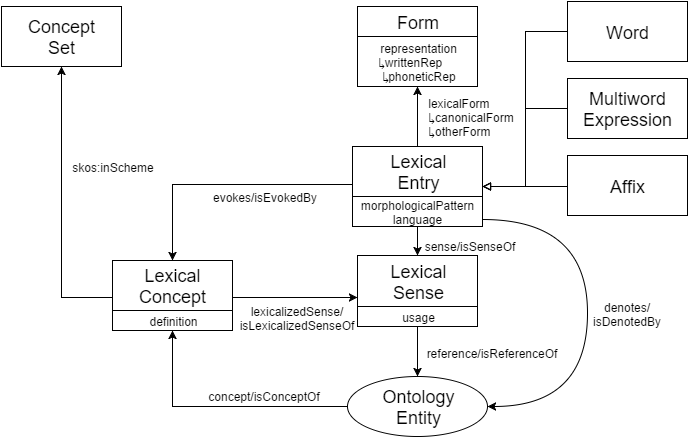
\includegraphics[width=0.8\textwidth]{Lemon_OntoLex_Core.png}
\caption{\label{fig:core}The Core Lemon OntoLex Model}
\end{figure}

The Lemon OntoLex model is based around the core module, as depicted in
Figure~\ref{fig:core}. The primary element of this is the \emph{lexical entry}
which represents a single word and thus collects together all morphological
expressions of that word, which correspond to \emph{forms} in the model, and all
possible concepts in the ontology it can refer to, which correspond to
\emph{lexical senses} in the model. It is important to note that the actual
meaning of a word is given by reference to an ontological concept and
\emph{lexical senses} represent only the mapping from a word to a concept. In
contrast to the previous lemon model, a third semantic element called the
\emph{lexical concept} was introduced that allows for a meaning to be defined
independently of an ontology. For example, the verb `to die' may refer to
ontological properties such as \texttt{deathDate} and \texttt{deathPlace} while
still referring to a single concept of \emph{Dying}. The model also supports
some other features including marking the canonical form (lemma), whether an
expression is a multiword expression and giving a \emph{usage} condition
describing when a particular word expresses a given concept (for example the
register), which is annotated on the lexical sense showing its role in giving a
mapping between concepts.



\section{Use cases}

\subsection{Representing dictionaries with OntoLex}

\subsection{The Collaborative Interlingual Index}

\section{Extensions and Future Plans}

\section{Conclusion}

\section*{Acknowledgement} 

Place all acknowledgements (including those concerning research grants and
funding) in a separate section at the end of the article.

\section*{References}

%\nocite{*}
\printbibliography[
    type={book},
    notkeyword={dictionary},
    title={Books}
]
\printbibliography[
    type={incollection},
    title={Book Sections}
]
\printbibliography[
    type={inproceedings},
    title={Paper in conference proceedings}
]
\printbibliography[
    type={article},
    title={Journal Articles}
]
\printbibliography[
    type={misc},
    title={Technical Reports}
]
\printbibliography[
    type={book},
    keyword={dictionary},
    title={Dictionaries}
]


\medskip
\begin{minipage}[t]{\textwidth}
    \noindent This work is licensed under the Creative Commons Attribution
    ShareAlike 4.0 International License.
    \vspace{-2ex}
    \begin{center}%
        \url{http://creativecommons.org/licenses/by-sa/4.0/}\linebreak
        
\includegraphics[width=2.33cm]{cc.png}%
    \end{center}
\end{minipage}

\end{document}
% vim: noai nocin nosi inde=:
